% "!TEX root = sprints.tex"
\noindent \large{\textbf{Summary}}\\
\normalsize Team Expeditus was unfortunately unable to complete the tasks for sprint 5, but the team was able to make measurable progress towards the goals. After deciding not to pursue simulation, the team members began to focus on message passing and offboard control between the flight controller and the Odroid. After multiple issues with multiple approaches to the AR tag tracking, the team was able to successfully get the AR Track Alvar library up and running.
\vspace{5mm}
\\
\noindent \Large{\textbf{Team Work}}
\normalsize
\begin{itemize}
\item \textbf{Jonathan Dixon:} Worked on AR tracking.
\item \textbf{Dylan Geyer:} Worked on AR tracking.
\item \textbf{Christopher Smith:} Worked on message passing and offboard control. 
\item \textbf{Steven Huerta:} Worked on AR tracking. 
\end{itemize}

\vspace{5mm}
\noindent \Large{\textbf{Uncompleted Tasks}}\\
\vspace{2mm}\\
\noindent \large{\textbf{As an owner, I want the UAV to autonomously land on the landing pad without damaging the craft}}
\normalsize
\begin{itemize}
\item \textbf{Modify/Rewrite implementation as necessary}
\begin{itemize}
\item \textbf{Visual Tracking by use of non-ROS version of AR tracker}\\
The team was able to successfully download, install, and run a non-ROS version of ALVAR to track AR Tags. The GUI elements of the AR Tracking program were removed and replaced by printing the quaternian and translation data of the AR Tag to the terminal.\par
The team decided not to pursue this any further since we were able to get the AR Track Alvar ROS package working which will save us the time of creating our own ROS wrapper around alvar.\par

\item \textbf{Visual Tracking by use of ROS version of AR tracker}\\
AR\_TRACK\_ALVAR is a package in ROS that provides AR tracking. This, as the name suggests, provides the ability to track AR tags. This is a ROS implementation of the ALVAR tool. Initially, this was the tool that the team wanted to use to estimate the UAV's pose relative to AR tag. This estimation is important, as it would allow the UAV to accurately estimate the location of the landing pad with the correct orientation. \par
The team, however, was unable to get this package functioning correctly. The documentation of the package is poor, and after struggling with making this package functional, we abandoned this path. However, after struggling with making the necessary components of ALVAR functional, we again attempted to use the ROS Package which that was available. After spending a full week stumbling through poor documentation, user forums, and tinkering with various launch files, we are now able to use the package.\par
\begin{figure}[h]
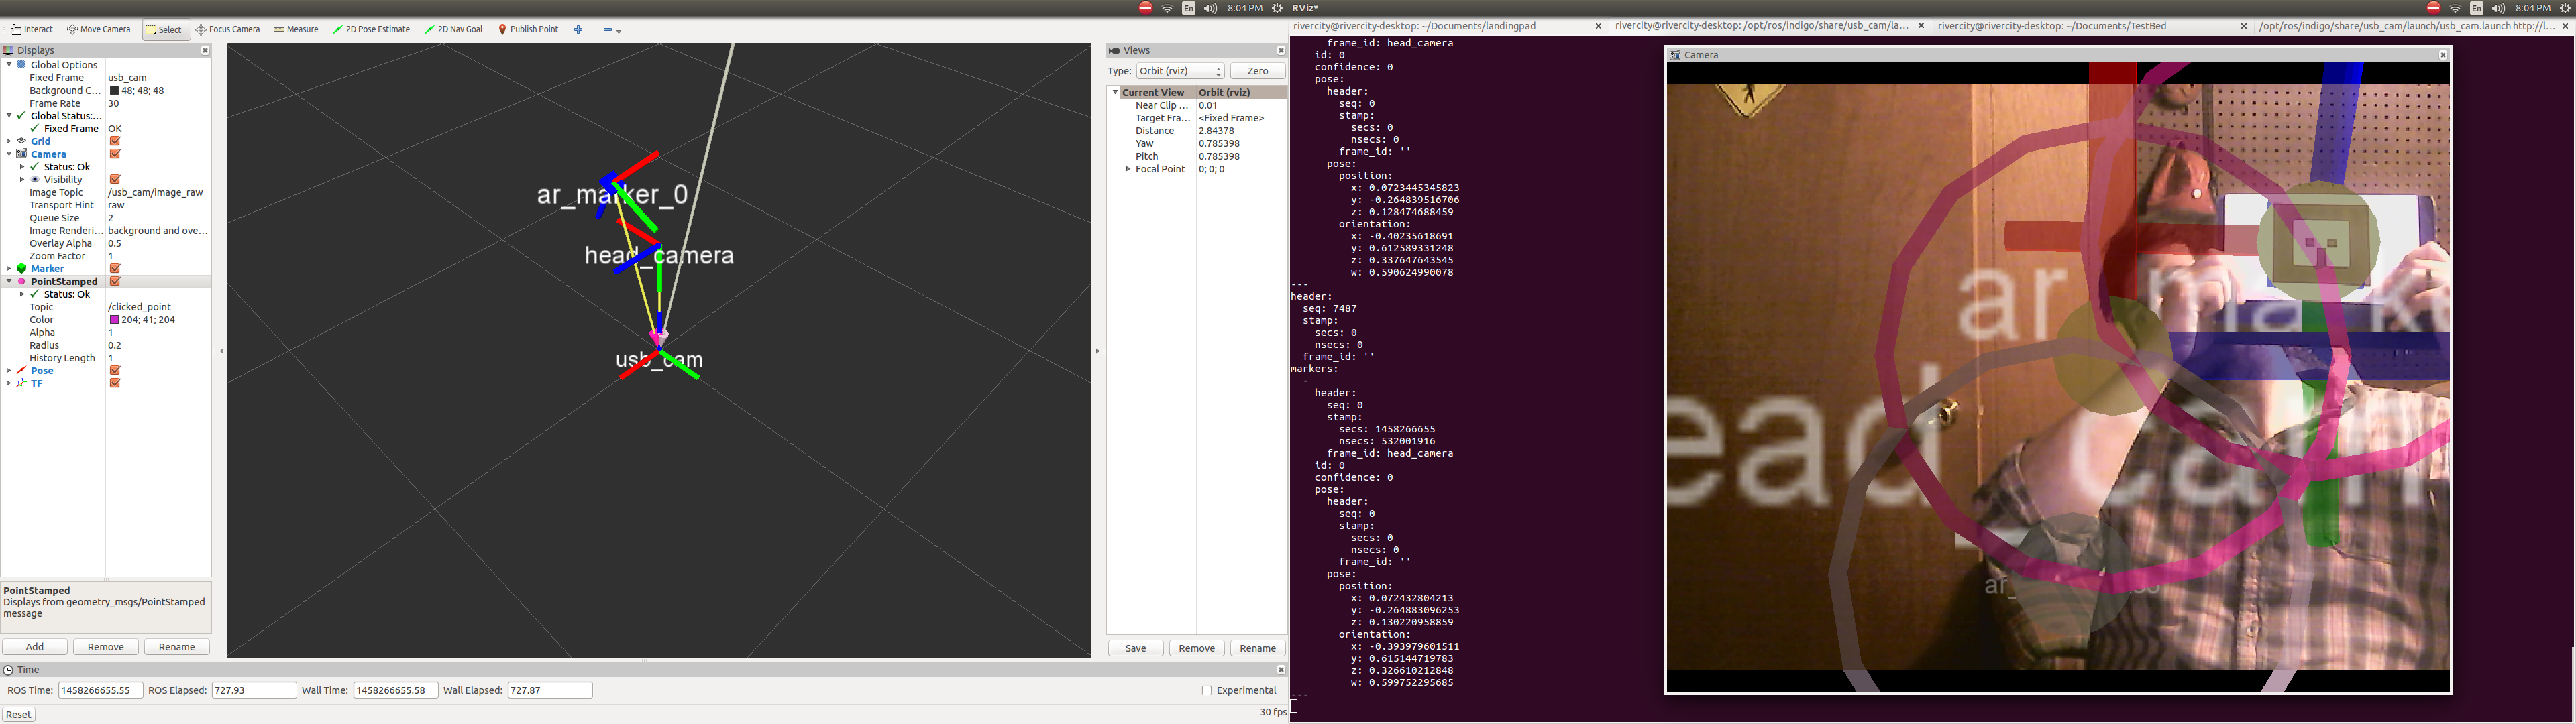
\includegraphics[width=7in]{artrackdemo.png}
\centering
\caption{ALVAR AR Tracker Demo in RViz}
\label{fig:artracker}
\end{figure}
This package will now serve as our means to relate the position of the UAV to the landing site, including orientation. As demonstrated in Fig.~\ref{fig:artracker}, this package provides AR tag identification, pose and orientation of the tag. We will use this information to provide our flight controller with necessary move commands to land the UAV.\par

\item \textbf{Offboard Local Control of UAV}\\
Offboard control was successfully achieved. After the successful flights using just QgroundControl and the pixhawk we attached the odroid to the uav on stands mounted right above the pixhawk. ROS Jade is installed on the ubuntu lts 14.04 odroid. Mavros is also installed and was able to connect to the pixhawk through USB and not throw any errors of connection.\par

\noindent Once we achieved this connectivity we wrote an simple offboard flight control node that would send location setpoints of a pose message in ROS composed of a position (x, y, z) and yaw. The first message that was tested was the position [0, 0, 0], and 0 yaw. When the drone was switched to offboard mode once setpoint data was being streamed nothing happened as was expected. The motors did not increase in velocity.\par

\begin{wrapfigure}{r}{0.25\textwidth} %this figure will be at the right
    \centering
    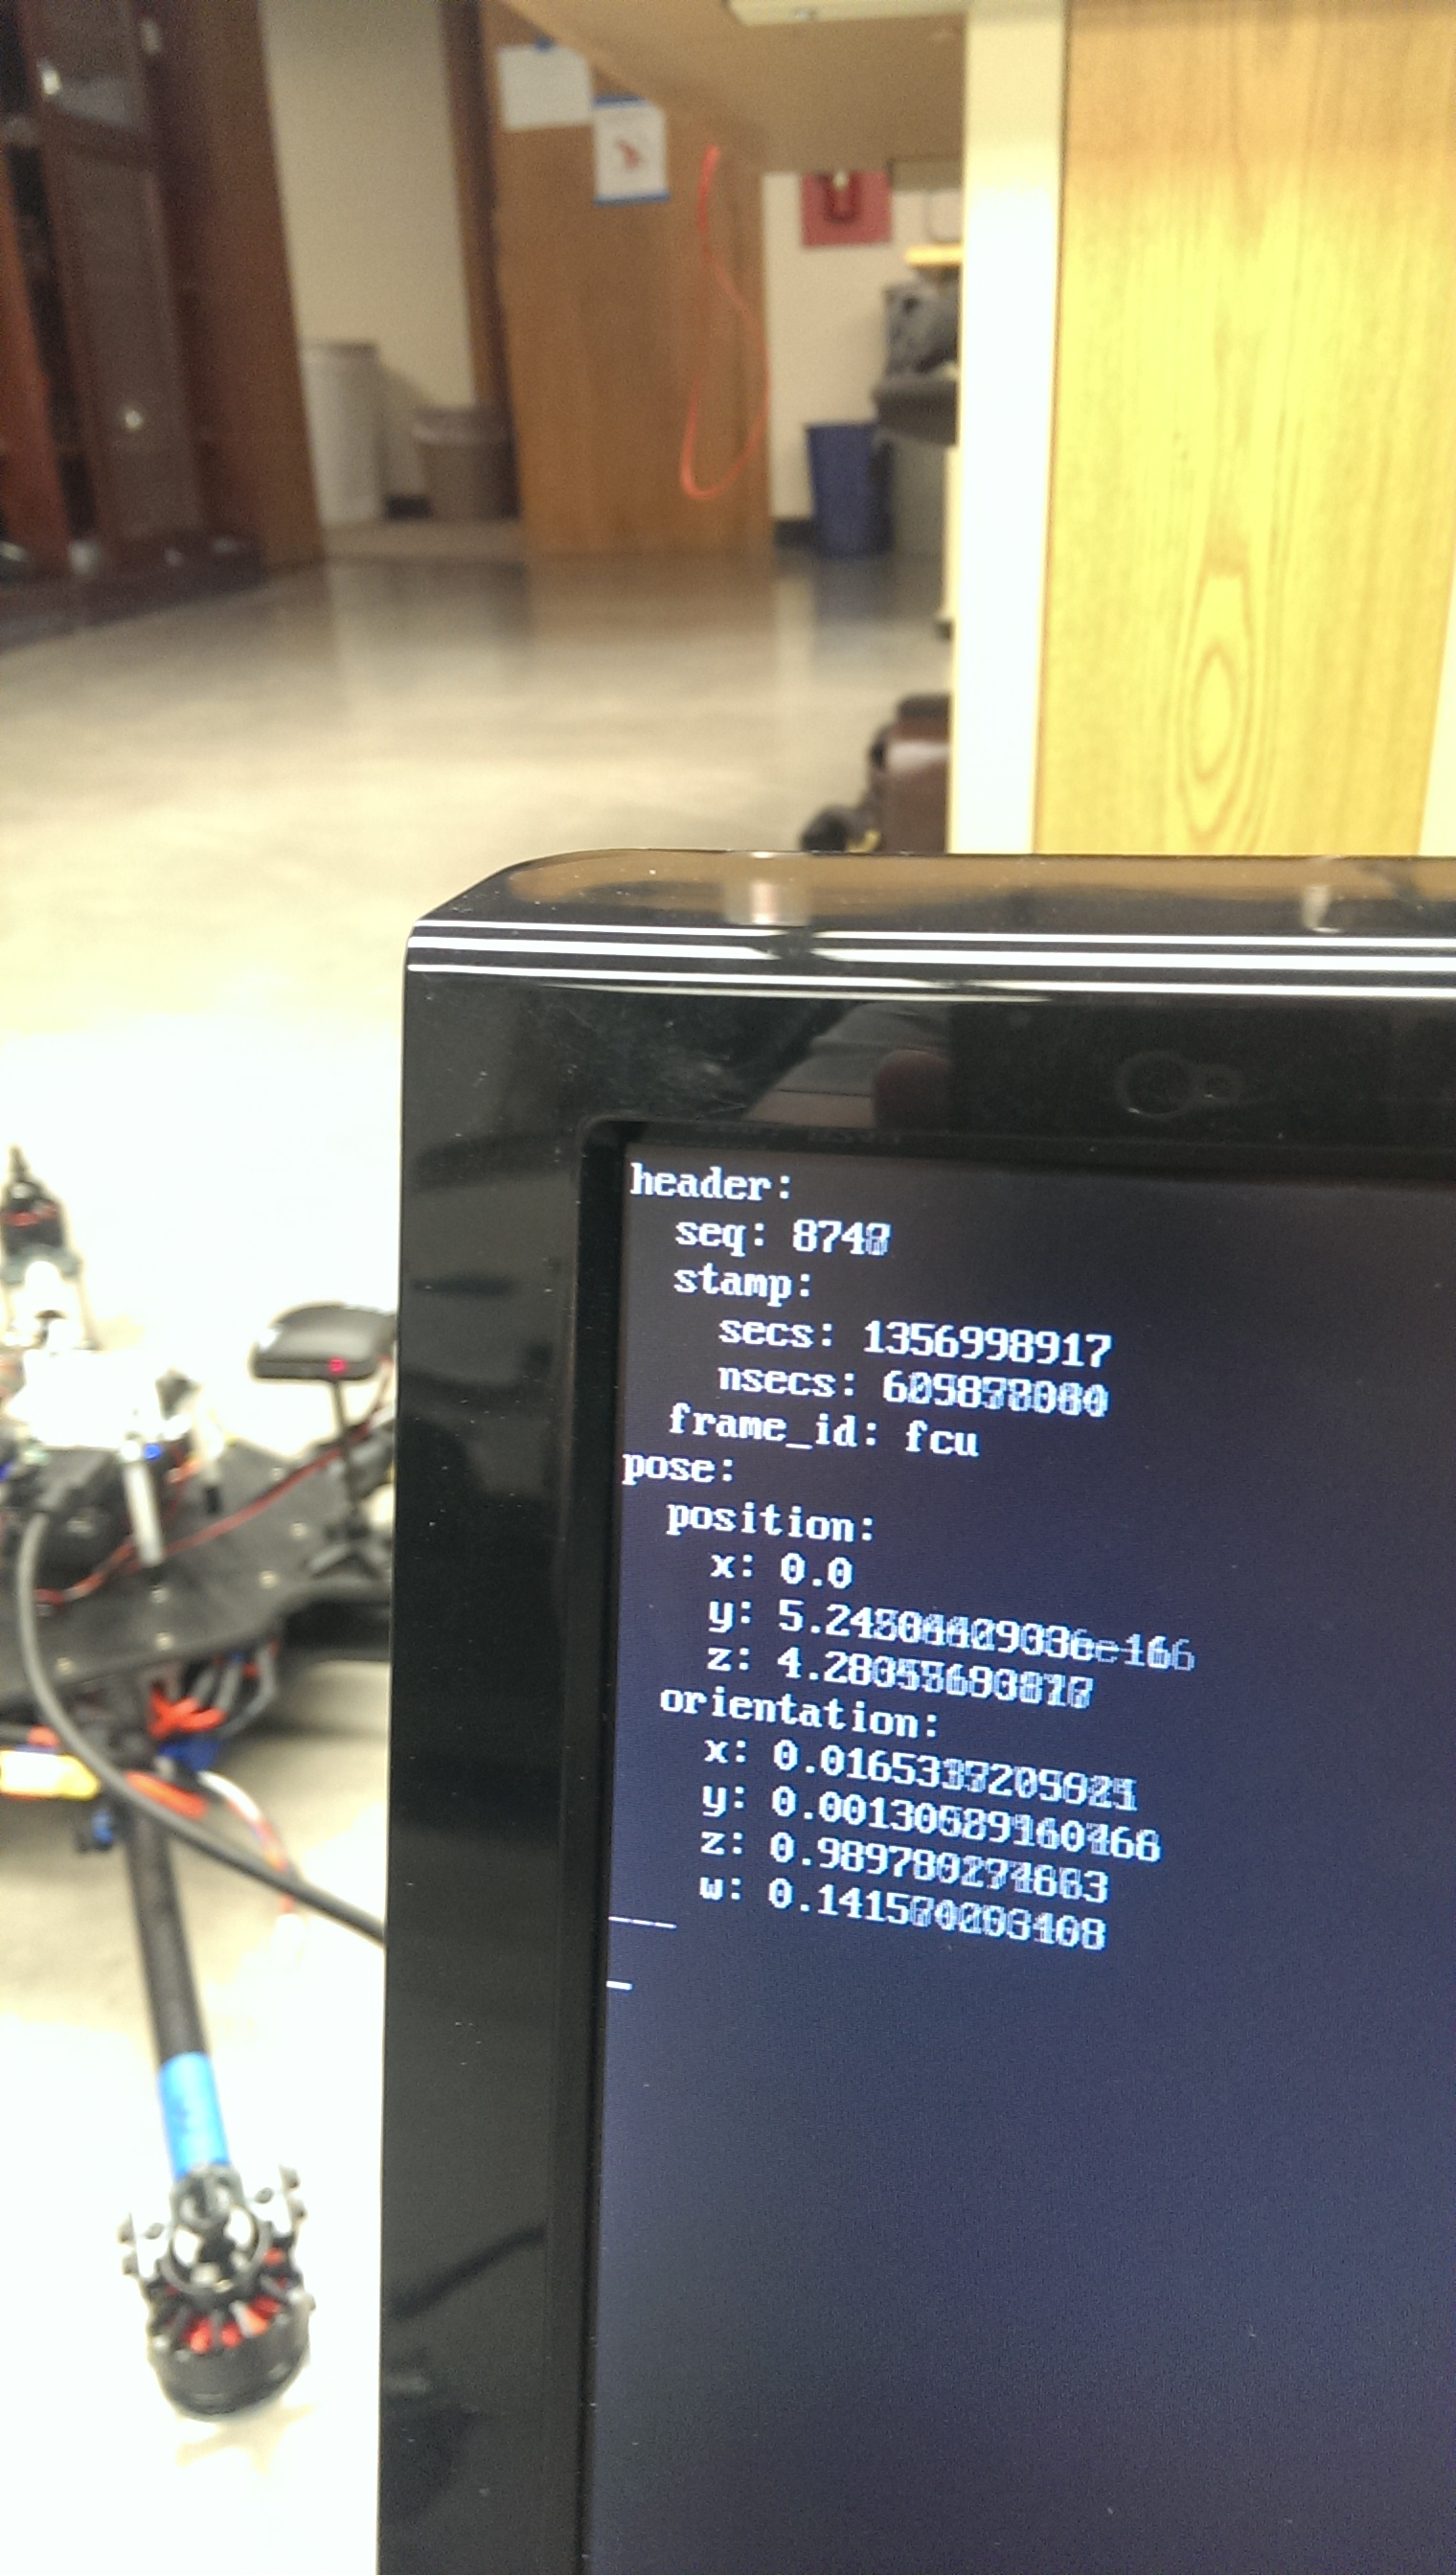
\includegraphics[width=0.25\textwidth]{messages.jpeg}
\end{wrapfigure}

\noindent The second test was to send a setpoint of [0, 0, 1], and 0 yaw. During this test the motors did increase in velocity significantly as the controller switched the uav from stabilize mode to offboard mode. We switched it back and forth between the two modes making sure all motors were increasing in speed. Once we did that we physically picked it up and moved it up and to the 1 meter mark. Once the setpoint position was either reached or passed the motors did slow down in speed to try and hold that position or lower itself to that position.\par

\noindent All the tests appeared to be working without monitoring the actual positions that were being streamed across the ROS topics. However, once we started looking at the data that was on the topics we noticed that where the uav started the local position topic would drift considerably in location. This issue was caused by being inside and in a basement. The x, y, and z location the pixhawk was reporting was not consistent. On some boot ups it would say it was at roughly [0, 0, -4] but the z value -4 would fluctuate severely by plus or minus 5. The x and y values would hover around the 0 marks usually but occasionally would fluctuate in the plus or minus 20 area. This was when we found that the onboard sensors would not be enough to perform at the fidelity we wanted in an ideal testing environment.\par

\noindent Once a nice day happened we took it outside to make sure that the building was the only severe drift effects on the sensors of the pixhawk. We took it out fifty feet from structures and performed the same tests on the uav as above. There were still errors but this time they were less but was off plus or minus a couple meters in all directions. The yaw appeared to have no issues or if it was off in the decimal places due to picking up the uav ourselves.\par 

\noindent Since all the onboard sensors would not provide us the fidelity in control that we wanted on their own we started researching different things to implement localization with the pixhawk sensors and exterior ones like a camera. So far it appears that visual odometry or optitrack are going to be the the best solutions to give us localization when we are above the landing pad. What still needs to be done is sending a pose estimate from the camera to the pixhawk using a kalman filter. We wish to treat the tag on the landing pad as the origin of the uav so that only setpoints that increasingly get it closer to [0, 0, 0] are sent.\par

\end{itemize}

\end{itemize}



\vspace{3mm}
\noindent \large{\textbf{As an owner, I want the UAV to autonomously land on the landing pad with the correct orientation.}}
\normalsize
\begin{itemize}
\item \textbf{Modify/Rewrite implementation as necessary}\\
As mentioned in the previous section, our team has not completed the tasks relating to the landing, which are dependent on:
\begin{itemize}
\item Estimate of Pose
\item Providing the commands to the flight controller to move the UAV to the landing pad.
\end{itemize}
AR\_TRACK\_ALVAR will provide estimation of the orientation of the AR tag relative to the camera. This will be used to correct the orientation of the craft. As message passing from and to the flight controller is solved through the use of MavROS, the team will now concentrate its efforts to correct issues offboard movement control. This, as mentioned previously, is the result of insufficient information for the flight controller to estimate its position.
\end{itemize}

